\section{Classifier}\label{sec:classifier}
As described in \cref{sec:machine_learning_task} we want to solve a supervised binary classification problem, and in order to do so we train a classifier. The previous section describes our feature extraction method. We will in this section describe how we use this method to extract features from training examples, and based on these choose a classification algorithm. We furthermore describe how we optimize the classifier's parameters to increase performance.

\subsection{Training Data}\label{sec:training_data}
Like all supervised learning, the classifier model is learned through training data.

As described in \ref{sec:choice_of_graph} we use featured articles and what they link to, to train the classifier. This data is split into 20\% test data and 80\% training data. This specific split is made to preserve the link structure in the graph while still having a reasonable amount of samples to test on. To train the classifier to find links that do not already exist, a random distribution of 50\% of the edges is removed from the training data. This ensures that we do not overfit the classifier on already existing links. \todo{Det er muligvis lidt dårligt forklaret mht. de 50\%}
%One sample of training data has the form \mono{<source article> <target article> <label>}. The source and targeet article are titles of pairs of articles. The label on the training samples can either be positive (link) or negative (do not link).

%Disjoint sets $P_{80} \subset P$ and $P_{20} \subset P$

As described in \cref{sec:machine_learning_task} we use a set of positive labeled training pairs $P$ and a set of negative labeled training pairs $N$. The positive training samples are pairs of linked articles as defined by $P$. As $\left\vert{P}\right\vert$ is smaller than $\left\vert{N}\right\vert$, we randomly sample from $N$ until we have as many negative as positive training pairs. Specifically for every positive pair $(a,b) \in P$, we randomly create a negative sample $(a,c) \in N$. A similar procedure is used for generating negative test samples, but it is also ensured that the random target article $c$ was not part of the training data.

%The positive samples are pairs of articles $(a,b)$ such that article $a$ is featured and there exists a link from article $a$ to $b$.



%We first experimented with negative samples being random article pairs $(a,b)$ fulfilling the condition of $N$: that article $a$ is featured and there does not exist a link from article $a$ to $b$. The problem with this approach is that it is too easy to overfit using these negative samples. As the article pairs are randomly sampled, most of the times, there is very little relatedness between the two articles. This is of course the point of a negative training sample, but because most of the negative samples were so unrelated, the classifiers used in our experiments could too easily differentiate positives from negatives. We needed another method that would give us negative samples where the articles have a higher likelihood of being related. Our second approach was to extract N-grams from all featured articles. Iterating through all N-grams for a featured article, a negative sample would be generated if another article had the exact same title as the N-gram, but the two article were not linked.

\subsection{Choosing a Classifier}\label{choosing_classifier}
To get a coarse estimate of which classifier seems the most appropriate for our purpose, we create a test harness that will run a range of classification algorithms on the same dataset. By comparing the algorithms against each other, we should be able to weed out the worst performing algorithms and get an approximate overview of the performance of each algorithm. Each algorithm will be run with its default parameters which is suboptimal, but finding good parameters for all algorithms is unrealistic given the time frame of this project. Based on the results, we choose the algorithm that looks the most promising to optimize further.

The examined algorithms are chosen mostly based on classifiers available in the scikit-learn Python library. There are many algorithms to choose from, and as all the algorithms are in the same library, the interface is the same, significantly simplifying the test harness.

\subsubsection{Evaluation Metrics}\label{evaluation_metric}
To evaluate the performance of each algorithm, we perform a 3-fold cross-validation. We deemed this sufficient compared to a 10-fold, because we are during a broad comparison and is able to produce results faster.
As the core of our problem definition is to produce reasonable suggestions of missing links, false positives should be punished harder than false negatives. A false positive is the suggestion of a link, that the classifier thinks should be there, but actually should not. A false negative is the suggestion of a link, that the classifier thinks should \emph{not} be there, but actually should. In other words, we believe it is worse to suggest a pair of articles to be linked that should not actually be linked, than not suggesting a pair of articles that should be linked. 

Because of the before mentioned higher penalty rate of false positives we want to favor precision over recall, as precision decreases as the number of false positives increases.

A common measure of a test's accuracy is the \emph{F-score}, which considers both precision and recall. Variants exists that weighs precision higher than recall, but because we want to minimize the amount false positives we choose to only consider precision as our evaluation metric.

\begin{equation}\label{eq:precision}
\text{Precision} = \frac{\text{true positives}}{\text{true positives} + \text{false positives}}
\end{equation}

\begin{equation}\label{eq:recall}
\text{Recall} = \frac{\text{true positives}}{\text{true positives} + \text{false negatives}}
\end{equation}


\subsubsection{Results}
A barchart of results can be seen in \cref{fig:classifier_comparison}. \emph{QDA} gives the best precision of $0.985$. However the recall is low, which is concerning as this means the number of suggestions are reduced. The next best result, \emph{Nearest Centroid}, gives a precision of $0.979$ which is also high, but with a far better recall. We would rather trade $0.6\%$ percent precision for much better recall, and therefore choose \emph{Nearest Centroid} as our classifier.

\todo{Skal vi vise en confusion matrix?}

%\begin{figure}[tbp]
%\centering
%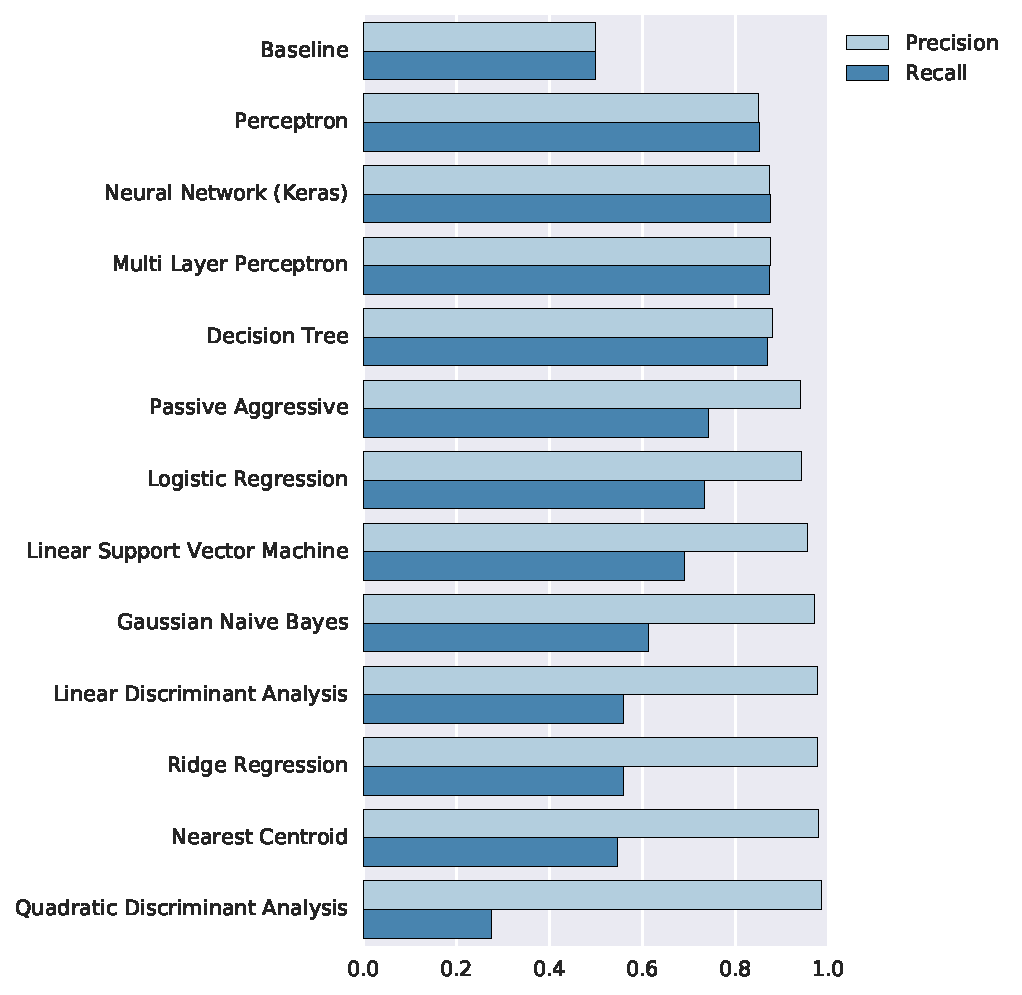
\includegraphics[width=0.95\textwidth]{classifier-comparison2.pdf}
%\caption[Precision and recall scores for the chosen algorithms]{Precision and recall scores for the chosen algorithms, sorted by precision.}\label{fig:classifier_comparison}
%\end{figure}

\begin{figure}%
\centering
\tikzsetnextfilename{barchart}
\begin{tikzpicture}
  \begin{axis}[
      table/col sep=semicolon,
      xbar=0pt, xmin=0, xmax=1,
      xlabel=Score,
      yticklabels from table={chapter_design/precision.csv}{name},
      %yticklabel style={text height=1.5ex},
      ytick=data,
      width=0.6\textwidth,
      y=0.9cm,
      enlarge y limits={abs=0.6},
      bar width=8pt,
      /pgf/number format/fixed,
      axis lines*=left,
      xmajorgrids=true,
      legend entries={Recall, Precision},
      legend style={draw=none},
      reverse legend, area legend,
      legend style={at={(1,1.01)},anchor=south east}
    ]
    \addplot [fill=color1!20!white] table [y expr=-\coordindex, x=recall] {chapter_design/precision.csv};
    \addplot [fill=color1!70!white] table [y expr=-\coordindex, x=precision] {chapter_design/precision.csv};
    
  \end{axis}
\end{tikzpicture}
\caption[Precision and recall scores for the chosen algorithms]{Precision and recall scores for the chosen algorithms, sorted by precision}\label{fig:classifier_comparison}%
\end{figure}

% \begin{table}[tbp]
% \centering
% \begin{tabular}{@{}lp{.75\textwidth}@{}}
% \toprule
% \textbf{Classifier} & \textbf{Result} \\
% \midrule
% Baseline           &  DummyClassifier()                \\
% Nearest Neighbors  &  KNeighborsClassifier(3)          \\
% Linear SVM         &  SVC(kernel="linear", C=0.025)    \\
% RBF SVM            &  SVC(gamma=2, C=1)                \\
% Gaussian Process   &  GaussianProcessClassifier        \\
% Decision Tree      &  DecisionTreeClassifier           \\
% Random Forest      &  RandomForestClassifier           \\
% Neural Net         &  MLPClassifier, KerasClassifier   \\
% AdaBoost           &  AdaBoostClassifier()             \\
% Naive Bayes        &  GaussianNB()                     \\
% QDA                &  QuadraticDiscriminantAnalysis()  \\
% \bottomrule
% \end{tabular}
% \caption[Classifiers]{Classifiers}%
% \label{tab:classifiers}
% \end{table}

\subsection{Parameter Optimization}
To attempt to further increase the performance of the chosen classifier, we optimize its parameters. The \emph{nearest centroid} implementation in the scikit-learn library does only have 2 parameters, so we choose to exhaust all parameter possibilities using grid search, as the parameter space is small.

Searching the parameter space reveals that the best parameters are the default parameters, also used above, where the distance metric is euclidean distance and no feature shrink threshold.

\todo{hvordan laver vi segway over mod ui afsnit? Michael spørger: Hvorfor er det nødvendigt med en segway?}
